% Suggested double-column placement. Requires graphicx in the manuscript.
% This snippet is supplied separately and has not been inserted into a main file.
\begin{figure*}[!t]
  \centering
  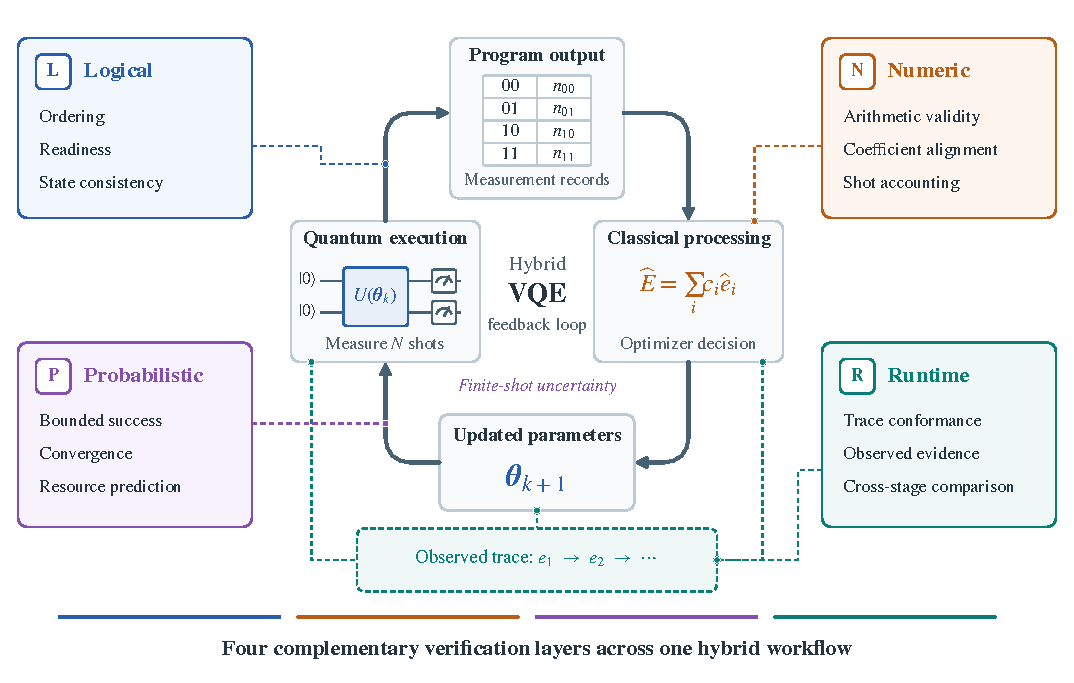
\includegraphics[width=\textwidth]{figures/introduction-overview.pdf}
  \caption{Hybrid VQE workflow and the complementary verification concerns that
  motivate the four-layer architecture. Quantum execution produces finite-shot
  measurement records. Classical processing constructs energy estimates and
  selects parameters for the next execution. Here $n_b$ denotes outcome counts
  from $N$ shots, and $\widehat E$ combines estimated Pauli expectations
  $\widehat e_i$ with Hamiltonian coefficients $c_i$. Logical checks address phase
  dependencies, numeric checks address arithmetic and accounting, and
  probabilistic analysis addresses bounded success, convergence, and resource
  use under stated assumptions. Runtime checking relates observed executions to
  specified obligations and prospective results. Probabilistic comparisons use
  repeated executions. Solid arrows show VQE data flow; dashed links indicate
  verification concerns and trace observations. The record contents are symbolic.}
  \label{fig:introduction-overview}
\end{figure*}
